\documentclass[12pt,a4paper]{report}

\usepackage[utf8]{inputenc}
\usepackage[romanian,english]{babel}
\renewcommand\familydefault{\sfdefault}

\usepackage[table,xcdraw]{xcolor}
\usepackage[margin=2.54cm]{geometry}
\usepackage{graphicx}

\usepackage{textcase}
\usepackage[titletoc, title]{appendix}
\usepackage{titlesec}
\titleformat{\chapter}{\large\bfseries\MakeUppercase}{\thechapter}{2ex}{}[\vspace*{-1.5cm}]
\titleformat*{\section}{\large\bfseries}
\titleformat*{\subsection}{\large\bfseries}
\titleformat*{\subsubsection}{\large\bfseries}

\usepackage{float}
\usepackage{microtype}
\usepackage{nicefrac}
\usepackage{amsfonts}
\usepackage{url}
\usepackage{multirow}
\usepackage{amssymb,amsmath,amsfonts,amsthm,bm}
\usepackage{tabularx}
\usepackage{listings}

\definecolor{codegray}{rgb}{0.5,0.5,0.5}
\definecolor{backcolour}{rgb}{0.95,0.95,0.92}

\lstdefinestyle{mystyle}{
    backgroundcolor=\color{backcolour},
    numberstyle=\tiny\color{codegray},
    basicstyle=\ttfamily\footnotesize,
    breakatwhitespace=false,
    breaklines=true,
    captionpos=b,
    keepspaces=true,
    numbers=left,
    numbersep=5pt,
    showspaces=false,
    showstringspaces=false,
    showtabs=false,
    tabsize=2
}
\lstset{style=mystyle}

\usepackage{chngcntr}
\counterwithout{figure}{chapter}
\counterwithout{table}{chapter}
\counterwithout{equation}{chapter}

\usepackage{booktabs}
\usepackage[bookmarks,unicode,hidelinks]{hyperref}

\usepackage{array}
\usepackage{paralist}
\usepackage{verbatim}
\usepackage{subfig}
\usepackage{enumitem}
\setlist{noitemsep}

%%% HEADERS & FOOTERS
\usepackage{fancyhdr}
\pagestyle{empty}
\renewcommand{\headrulewidth}{0pt}
\renewcommand{\footrulewidth}{0pt}
\lhead{}\chead{}\rhead{}
\lfoot{}\cfoot{\thepage}\rfoot{}

\newcommand{\HeaderLineSpace}{-0.25cm}
\newcommand{\UniTextEN}{UNIVERSITY POLITEHNICA OF BUCHAREST \\[\HeaderLineSpace]
FACULTY OF AUTOMATIC CONTROL AND COMPUTERS \\[\HeaderLineSpace]
COMPUTER SCIENCE AND ENGINEERING DEPARTMENT\\}
\newcommand{\DiplomaEN}{Scientific Report \#4}
\newcommand{\AdvisorEN}{Scientific advisors:}
\newcommand{\BucEN}{BUCHAREST}

\newcommand{\frontPage}[6]{
\begin{titlepage}
\begin{center}
{\Large #1}
\vspace{50pt}
\begin{tabular}{p{6cm}p{4cm}}

\includegraphics[scale=0.8]{figures/upb-logo.jpg} &
	
\includegraphics[scale=0.5,trim={14cm 11cm 2cm 5cm},clip=true]{figures/cs-logo.pdf}
\end{tabular}

\vspace{105pt}
{\Huge #2}\\
\vspace{40pt}
{\Large #3}\\ \vspace{0pt}
{\Large #4}\\
\vspace{40pt}
{\LARGE \Name}\\
\end{center}
\vspace{60pt}
\begin{tabular*}{\textwidth}{@{\extracolsep{\fill}}p{6cm}r}
&{\large\textbf{#5}}\vspace{10pt}\\
&{\large \AdvisorA}\\
&{\large \AdvisorB}
\end{tabular*}
\vspace{20pt}
\begin{center}
{\large\textbf{#6}}\\
\vspace{0pt}
{\normalsize \Year}
\end{center}
\end{titlepage}
}

\newcommand{\frontPageEN}{\frontPage{\UniTextEN}{\DiplomaEN}{\ProjectTitleEN}{\ProjectSubtitleEN}{\AdvisorEN}{\BucEN}}

\linespread{1.15}
\setlength\parindent{0pt}
\setlength\parskip{.28cm}

\newcommand{\AbstractPage}{
\begin{titlepage}
\textbf{\large ABSTRACT}\par
\AbstractEN \vfill
\end{titlepage}
}

\tolerance=1
\emergencystretch=\maxdimen
\hyphenpenalty=10000
\hbadness=10000
\sloppy

%%%%%%%%%%%%%%%%%%%%%%%%%%%%%%%%%%%%%%%%%%%%%%%%%%

\newcommand{\ProjectTitleEN}{Cross-Lingual and Large Language Model Approaches to Aspect-Based Sentiment Analysis}
\newcommand{\ProjectSubtitleEN}{Master Program IISC}
\newcommand{\Name}{[TO DO]}
\newcommand{\AdvisorA}{[TO DO]}
\newcommand{\AdvisorB}{}
\newcommand{\Year}{2026}

\title{Raport de cercetare}
\author{\Name}
\date{\Year}

\newcommand{\AbstractEN}{This report extends our previous work on out-of-domain generalisation in generative ABSA by investigating two complementary directions: the use of large language models in few-shot settings and the application of fine-tuned models to Romanian, a language with limited ABSA resources. We evaluate three LLMs (Gemma2 27B, Qwen2.5 32B, Command-R) in zero-shot and six-shot configurations on both the English SemEval ASTE benchmark and a Romanian aspect-based sentiment dataset (eMAG phone reviews). We compare their performance against fine-tuned models of varying sizes and language specialisation: FLAN-T5-base (250M, English-centric), XLM-R-base (278M, multilingual), and two Romanian-specific BERT models (RoBERT-base 114M, bert-base-romanian-cased 110M). Our findings indicate that fine-tuned models at 110--278M parameters consistently match or outperform 27--32B parameter LLMs in few-shot settings on both English extraction tasks and Romanian classification tasks. Among the Romanian models, we observe that monolingual pre-training provides an advantage over multilingual models for this specific task.}

\begin{document}

\frontPageEN

\begingroup
\linespread{1}
\tableofcontents
\endgroup

\AbstractPage


\chapter{Introduction}\label{ch:introduction}\pagestyle{fancy}

\section{Summary of Previous Work}

In a previous report, we presented an empirical study of training strategies for out-of-domain generalisation in generative Aspect-Based Sentiment Analysis. We formulated Aspect Sentiment Triplet Extraction (ASTE) as a sequence-to-sequence problem using FLAN-T5-base (250M parameters) and evaluated the effect of output format, syntactic input enrichment, multi-ordering training, sub-task decomposition, curriculum learning, aspect masking, cross-domain data mixing, and decoding strategies on cross-domain performance.

The main finding was that natural-language output templates provide the largest improvement for OOD generalisation: +8.6 F1 points over structured output (5 seeds, non-overlapping confidence intervals). On the DMASTE multi-domain benchmark, our model matched the best previously reported cross-domain result (Span-ASTE~\cite{xu2023dmaste}) without any domain adaptation. Most other interventions (syntax enrichment, curriculum learning, aspect masking, data mixing, task decomposition) did not reliably help. The common pattern was that strategies which increase training variety within the same domain do not address the vocabulary and annotation style differences that characterise cross-domain transfer.

That work focused exclusively on English and on the generative T5-based approach. Two questions remained open: how does a fine-tuned 250M model compare against much larger language models that have seen far more diverse pre-training data, and whether the findings extend to languages other than English where annotated ABSA data is scarce.


\section{Motivation}

This report addresses both questions. On the LLM side, we evaluate Gemma2 27B, Qwen2.5 32B, and Command-R (35B) in zero-shot and six-shot settings on the same SemEval ASTE task used previously. The comparison is straightforward: can a model with 100$\times$ more parameters, but no task-specific training, outperform a small fine-tuned model on structured extraction?

On the multilingual side, we evaluate on Romanian using a dataset of eMAG phone reviews annotated for aspect polarity and category. Romanian is a medium-resource language: pre-trained models exist (RoBERT~\cite{masala2020robert}, bert-base-romanian-cased~\cite{dumitrescu2020birth}) but fine-grained ABSA datasets are rare. This setting lets us compare several approaches: monolingual Romanian models (110--114M), a multilingual encoder (XLM-R, 278M), an English-centric generative model fine-tuned on Romanian data (FLAN-T5, 250M), and large language models prompted in Romanian without any fine-tuning.

The practical question is: for a practitioner with limited ABSA data in a non-English language, what is the most effective approach? Fine-tune a small monolingual model, fine-tune a multilingual model, fine-tune an English generative model, or prompt a large model with a few examples?


\section{Objectives}

\begin{enumerate}
    \item Compare large language models (27--35B parameters, few-shot) against fine-tuned models (110--278M parameters) on English ASTE extraction.

    \item Evaluate the same LLMs on Romanian ABSA (polarity + category prediction on eMAG phone reviews).

    \item Compare monolingual Romanian models (RoBERT-base, bert-base-romanian-cased) against multilingual (XLM-R-base) and English-centric generative (FLAN-T5-base) approaches on the same Romanian task.

    \item Discuss the role of LLM-generated annotations in low-resource ABSA settings, given that our Romanian training data was produced with GPT-4 assistance.
\end{enumerate}


\section{Structure}

Chapter~\ref{ch:relatedwork} reviews the relevant literature on multilingual models, LLMs for ABSA, and Romanian NLP. Chapter~\ref{ch:methodology} describes the experimental setup. Chapter~\ref{ch:implementation} covers the datasets and implementation details. Chapter~\ref{ch:results} presents results and analysis. Chapter~\ref{ch:conclusions} summarises findings.



\chapter{Related Work}\label{ch:relatedwork}

Two pre-trained language models exist specifically for Romanian. Masala et al.~\cite{masala2020robert} (COLING 2020) introduced RoBERT, a BERT model trained from scratch on Romanian text. They released three sizes: RoBERT-small (19M parameters), RoBERT-base (114M), and RoBERT-large (341M), all uncased. The training corpus consists of approximately 12GB of cleaned Romanian text from OSCAR, RoTex, and Wikipedia. On downstream tasks such as part-of-speech tagging and named entity recognition, RoBERT outperformed multilingual BERT by a considerable margin, demonstrating the value of monolingual pre-training even at the base model scale. Dumitrescu et al.~\cite{dumitrescu2020birth} (EMNLP 2020 Findings) independently trained another Romanian BERT, bert-base-romanian-cased, on a 15GB corpus comprising OPUS, OSCAR, and Wikipedia data. Their model is cased (unlike RoBERT which is uncased) and also outperformed multilingual BERT on Romanian benchmarks. Both papers report that language-specific pre-training on even moderately-sized corpora produces models that outperform multilingual alternatives on downstream tasks in that language. We use both models in our experiments as monolingual baselines for Romanian ABSA.

On the multilingual side, XLM-RoBERTa~\cite{conneau2020unsupervised} (XLM-R) is a transformer model trained on 2.5TB of filtered CommonCrawl data in 100 languages. At the base scale (278M parameters), it provides competitive performance across many languages without language-specific training. The trade-off is that its capacity is spread across 100 languages, so for any single language it has seen less language-specific data than a dedicated monolingual model, but it benefits from cross-lingual transfer. For Romanian specifically, XLM-R has been used as a backbone for various NLP tasks but its performance relative to the monolingual Romanian models on fine-grained tasks like ABSA has not been systematically compared.

The question of whether large language models can perform ABSA without fine-tuning has been investigated in several recent papers. Simmering and Huoviala~\cite{veyseh2024llm_absa} evaluated GPT-3.5 and GPT-4 on the SemEval 2014 joint aspect term extraction and polarity classification task and found that fine-tuned GPT-3.5 achieves state-of-the-art performance (83.8 F1), while GPT-4 in 6-shot settings reaches 71.3 F1 --- below fine-tuned smaller models. A consistent finding is that LLMs perform better at classification (determining whether something is positive or negative) than at extraction (identifying which specific words constitute an aspect or opinion span). This matches what we observe in our experiments: LLMs achieve reasonable aspect-level F1 but full triplet F1 drops substantially because opinion span matching is difficult without fine-tuning.

\v{S}m\'{i}d et al.~\cite{smid2024multilingual_llm_absa} (2024) conducted a systematic evaluation of LLMs for zero-shot multilingual ABSA across several languages. Their results indicate that while LLMs show promise, they generally fall short of fine-tuned task-specific models. They also found that simpler zero-shot prompts often outperform more complex prompting strategies, especially in high-resource languages. This is relevant context for our experiments: we use a straightforward structured prompt rather than elaborate chain-of-thought reasoning, and our results are consistent with their finding that fine-tuned models retain an advantage.

The same group~\cite{smid2025czech_absa} (2025) applied this comparison to Czech, a medium-resource language comparable to Romanian. They found that small domain-specific models fine-tuned for ABSA outperform general-purpose LLMs in zero-shot and few-shot settings. This parallels our Romanian findings and suggests the pattern is not language-specific but reflects a general property of extraction tasks: task-specific fine-tuning remains more sample-efficient than scaling model size for structured prediction.

On the cross-lingual ABSA front, recent work~\cite{fewshot_crosslingual_absa2025} has shown that adding as few as ten target-language examples to a sequence-to-sequence model significantly improves performance over zero-shot cross-lingual transfer. This is consistent with our setup: we fine-tune FLAN-T5-base on a small Romanian dataset rather than relying on zero-shot transfer from English, and it performs competitively with much larger models. A broader survey of cross-lingual transfer strategies for ABSA~\cite{crosslingual_transfer_absa2026} confirms that the field remains largely English-focused, and that practical approaches for non-English languages typically involve some amount of target-language fine-tuning rather than relying purely on zero-shot transfer.

A separate but relevant question concerns the use of LLMs as annotators for training data creation. Aldeen et al.~\cite{aldeen2023chatgpt} (ICMLA 2023) compared ChatGPT annotations against human annotators across several NLP tasks and found that LLM-generated annotations achieve competitive quality for sentiment analysis, though human annotators consistently outperform on more complex tasks requiring nuanced judgement. This is directly relevant to our setup: the Romanian eMAG training dataset was annotated with GPT-4 assistance (aspect categories and polarities generated by GPT-4, then reviewed). The quality of this annotation process affects the ceiling of what any model trained on it can achieve. We discuss this further in the results chapter.

For our generative approach on Romanian, we use FLAN-T5-base~\cite{chung2022scaling}, which was instruction-tuned primarily on English tasks. Despite being English-centric, FLAN-T5's tokenizer (SentencePiece) covers Romanian characters, and the model can generate Romanian text with fine-tuning. The question is whether this English-centric model, fine-tuned on a small Romanian dataset, can compete with models that have dedicated Romanian pre-training. Our previous report established that the natural-language output format~\cite{zhang2021aspect} helps OOD generalisation in English; here we test whether that benefit extends to a cross-lingual setting where the model generates text in a language it was not primarily designed for.



\chapter{Methodology}\label{ch:methodology}

This chapter describes the models, prompting strategies, and evaluation metrics used in our experiments.

\section{Models}

\subsection{Large Language Models (Few-Shot)}

We evaluate three LLMs via the ollama inference server, all 4-bit quantised:

\begin{itemize}
    \item \textbf{Gemma2 27B}~\cite{team2024gemma} --- Google's 27B parameter model.
    \item \textbf{Qwen2.5 32B}~\cite{hui2024qwen2} --- Alibaba's 32B parameter model.
    \item \textbf{Command-R}~\cite{cohere2024commandr} --- Cohere's 35B parameter model, designed for retrieval-augmented generation.
\end{itemize}

Each model is tested in 0-shot (task description only) and 6-shot (task description plus 6 demonstration examples) settings. For the 6-shot setting, demonstrations are retrieved from the training set using a hybrid strategy: 3 examples via BM25 (lexical similarity to the test sentence) and 3 via SimCSE (semantic similarity), ensuring both vocabulary and structural diversity.

\subsection{Fine-Tuned Classifier Models (Romanian)}

For Romanian polarity + category classification, we compare three encoder-based models:

\begin{itemize}
    \item \textbf{RoBERT-base}~\cite{masala2020robert} --- 114M parameters, Romanian-only, uncased.
    \item \textbf{bert-base-romanian-cased}~\cite{dumitrescu2020birth} --- 110M parameters, Romanian-only, cased.
    \item \textbf{XLM-R-base}~\cite{conneau2020unsupervised} --- 278M parameters, multilingual (100 languages).
\end{itemize}

All use the same classifier architecture: the encoder produces a sentence representation which is passed through linear heads for polarity classification and category classification. Training uses AdamW with a learning rate of $2 \times 10^{-5}$, 8 epochs, and early stopping with patience 3.

\subsection{Fine-Tuned Generative Model (Romanian)}

FLAN-T5-base~\cite{chung2022scaling} (250M parameters) is fine-tuned on the Romanian eMAG training set using natural-language output templates, following the same approach as our English experiments. The model generates text like ``polarity is positive, category is performance'' given a Romanian input sentence.


\section{Few-Shot Prompt Design}

For the English ASTE task, the LLM receives:

\begin{lstlisting}
Extract all (aspect, opinion, polarity) triplets from the sentence.
Polarity is one of: positive, negative, neutral.
Output format: [aspect, opinion, polarity]

Sentence: But the staff was so horrible to us .
Output:
\end{lstlisting}

In the 6-shot setting, 6 example input-output pairs precede the test sentence.

For Romanian, the prompt requests polarity and category extraction with the category taxonomy provided in the system prompt. Demonstrations (when used) are Romanian sentences from the training set.


\section{Evaluation}

For English ASTE, we use micro-averaged triplet F1 (exact match on all three elements), consistent with our previous report.

For Romanian, we report three metrics:
\begin{itemize}
    \item Polarity + Category pair F1 (both must match for a correct prediction).
    \item Polarity F1 (polarity alone).
    \item Category F1 (category alone).
\end{itemize}

This decomposition helps identify whether errors come from polarity classification (relatively easy) or category prediction (harder, especially for LLMs unfamiliar with the specific taxonomy).



\chapter{Implementation}\label{ch:implementation}

\section{Datasets}

We evaluate on two tasks across two languages:

\begin{enumerate}
    \item \textbf{English ASTE} (SemEval): Aspect Sentiment Triplet Extraction on restaurant/laptop reviews. Train on Rest14 (1266 sentences), test on Rest14 (in-domain), Rest15, Rest16, and Laptop14 (out-of-domain). This is the same setup as our previous report, now used to compare LLMs against the fine-tuned baseline.

    \item \textbf{Romanian ABSA} (eMAG): Joint polarity and category prediction on phone reviews from eMAG (a Romanian e-commerce platform). The task is to predict (polarity, category) pairs for each annotated aspect in a review sentence. Categories are drawn from a fixed taxonomy of 11 classes (experience, durability, performance, battery, price\_quality, design, camera, audio, software, brand, service). Polarities are positive, negative, or neutral. The training set was produced with GPT-4 assistance: reviews were processed by GPT-4 to identify aspects and assign polarity/category labels from the predefined taxonomy, followed by human review. The test set was annotated independently.
\end{enumerate}

Figures~\ref{fig:r4-polarity}--\ref{fig:r4-sentlen} characterise the Romanian dataset. The training set contains 27,630 sentences with 90,778 annotations (3.29 per sentence on average), drawn from a vocabulary of 65,188 unique words. Sentences are considerably longer than in the English SemEval data: mean 43.5 words (median 23), with a long tail reaching up to 309 words. At the subword token level (T5 tokenizer), the mean is 73.6 tokens (median 39, P95 = 266). The polarity distribution is heavily skewed toward positive (72.4\%), with negative at 22.6\% and neutral at only 5.0\%. The most frequent category is ``experience'' (25.7\%), followed by ``performance'' (11.5\%) and ``battery'' (10.3\%). The test set (3,093 sentences, 9,478 annotations) follows similar distributions, with slightly shorter sentences (mean 36.1 words) and a slightly higher neutral proportion (8.7\%).

\begin{figure}[H]
\centering
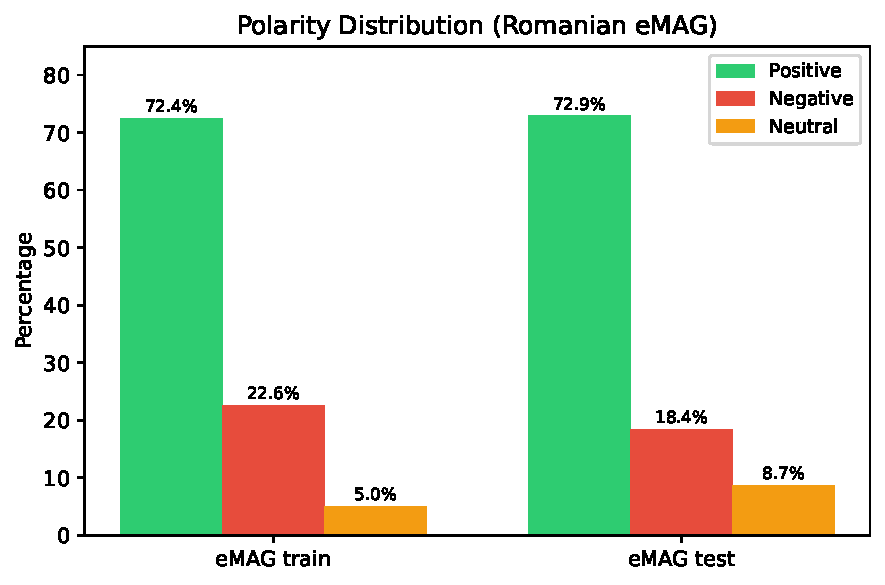
\includegraphics[width=0.7\textwidth]{figures/r4_polarity_distribution.pdf}
\caption{Polarity distribution in the Romanian eMAG training and test sets.}
\label{fig:r4-polarity}
\end{figure}

\begin{figure}[H]
\centering
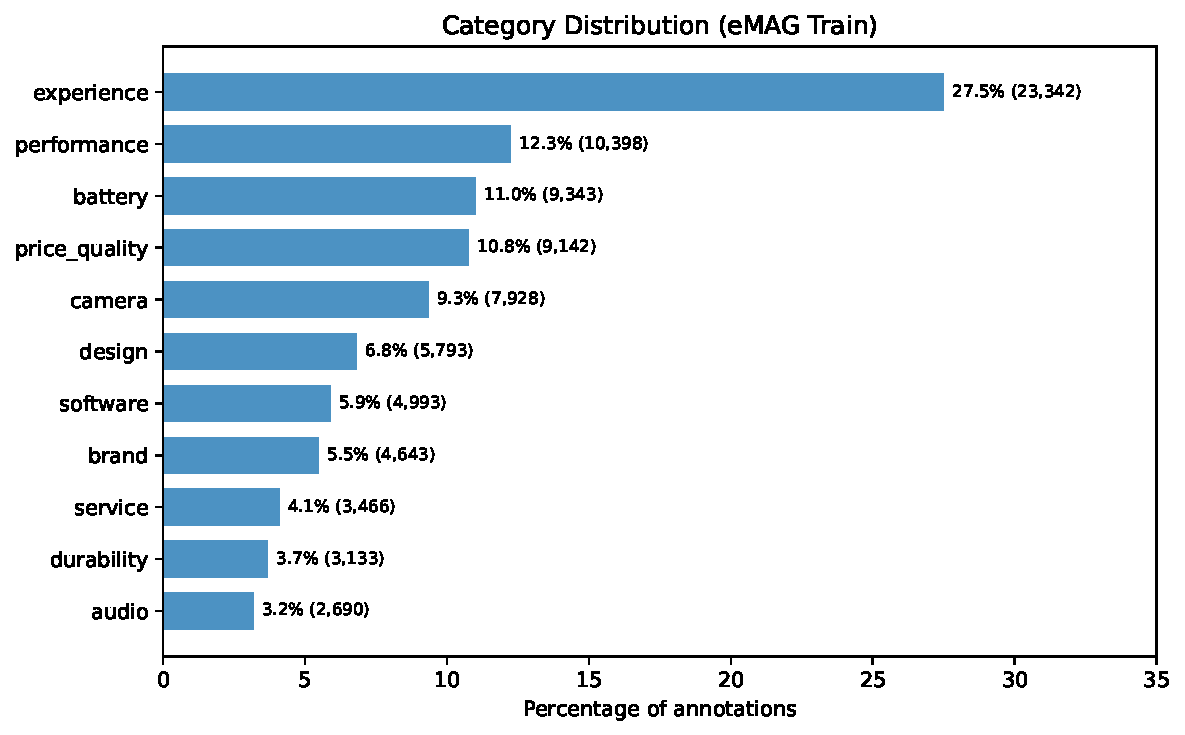
\includegraphics[width=0.85\textwidth]{figures/r4_category_distribution.pdf}
\caption{Category distribution in the Romanian eMAG training set (11 classes).}
\label{fig:r4-categories}
\end{figure}

\begin{figure}[H]
\centering
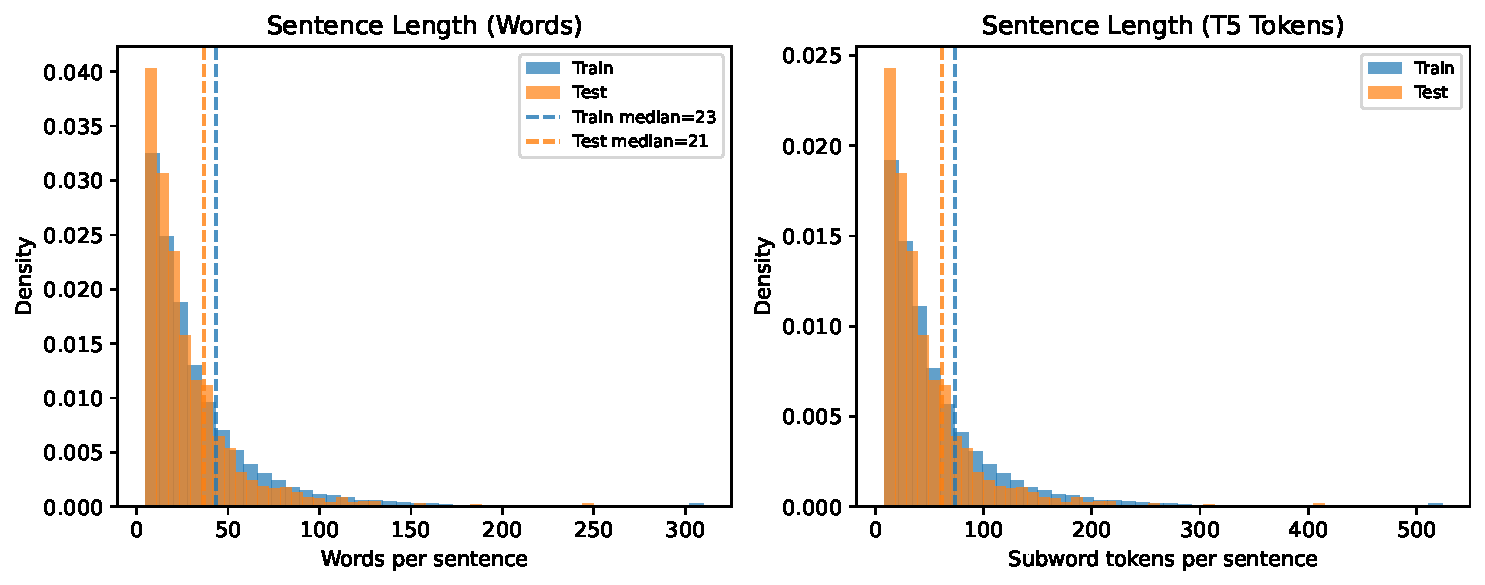
\includegraphics[width=0.95\textwidth]{figures/r4_sentence_length_histogram.pdf}
\caption{Sentence length distributions for the Romanian eMAG dataset at word and subword token level.}
\label{fig:r4-sentlen}
\end{figure}

\section{LLM Inference}

We use the ollama inference server to run quantised models locally. All three LLMs (Gemma2 27B, Qwen2.5 32B, Command-R) are loaded in 4-bit quantisation. Inference is performed sequentially on each test sentence. For the 6-shot setting, the hybrid demonstration retrieval combines BM25 (via rank-bm25) and SimCSE (via sentence-transformers) to select 3 lexically similar and 3 semantically similar examples from the training set. This ensures demonstrations cover both vocabulary overlap and structural similarity with the test sentence.

Output parsing follows the same strict protocol as our fine-tuned models: generated text is matched against expected patterns, and malformed outputs score zero. For English ASTE, we parse bracketed triplets; for Romanian, we parse polarity-category pairs from the generated text.

Figure~\ref{fig:pipeline-r4} shows the three parallel evaluation paths used in this report.

\begin{figure}[p]
\centering
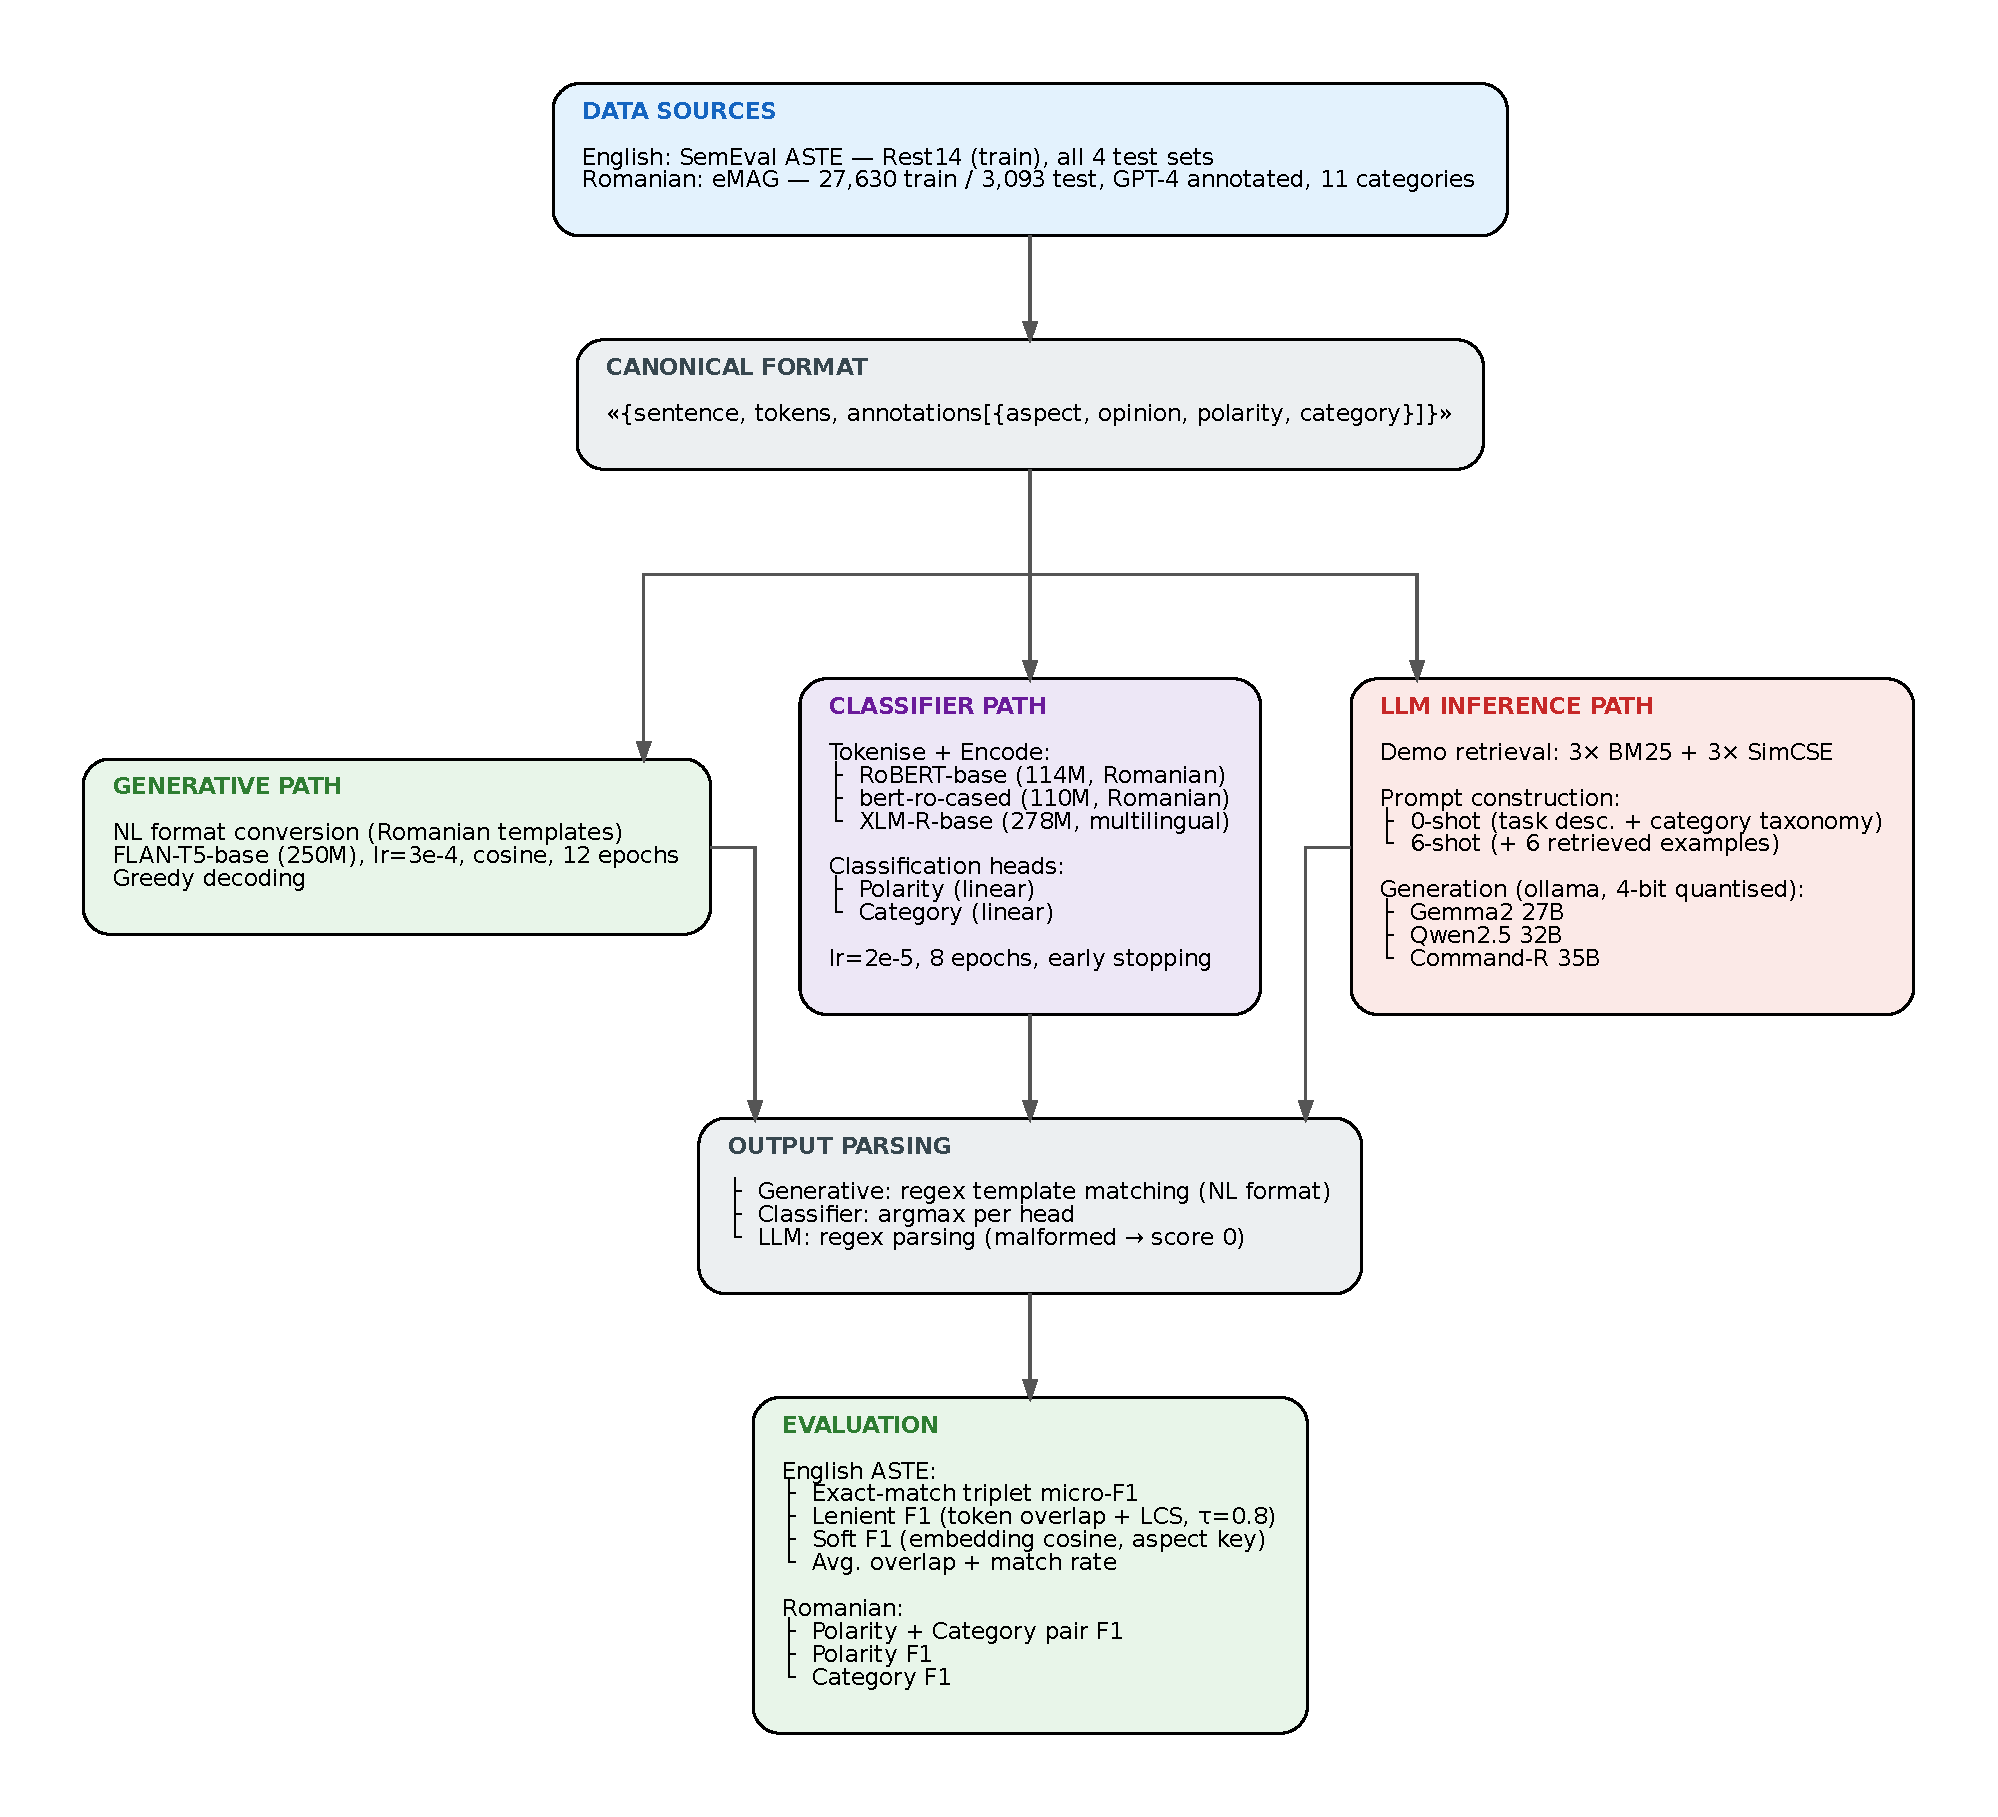
\includegraphics[width=\textwidth, height=0.88\textheight, keepaspectratio]{figures/pipeline_report4.pdf}
\caption{Evaluation pipeline showing the three parallel model paths: generative (FLAN-T5), classifier (BERT variants), and LLM inference.}
\label{fig:pipeline-r4}
\end{figure}

\section{Classifier Models}

The encoder-based classifiers (RoBERT, bert-ro, XLM-R) share the same architecture: the input sentence is tokenised, passed through the encoder, and the \texttt{[CLS]} token representation is used as input to two linear classification heads (one for polarity, one for category). The model is trained with cross-entropy loss on both heads simultaneously.

All classifiers use the same hyperparameters: learning rate $2 \times 10^{-5}$, weight decay 0.01, warmup ratio 0.06, batch size 16, gradient clipping at 1.0, bf16 mixed precision, and up to 8 epochs with early stopping (patience 3 on validation F1). A 10\% validation split is held out from the training data.

\section{Generative Model (Romanian)}

FLAN-T5-base is fine-tuned on the Romanian training set with natural-language output templates. The setup mirrors our English experiments: learning rate $3 \times 10^{-4}$, cosine schedule, 12 epochs (fewer than English due to the smaller dataset), effective batch size 32. The model generates Romanian-language output following a fixed template structure, which is then parsed back into polarity-category pairs.



\chapter{Experimental Results}\label{ch:results}

\section{LLMs on English ASTE}\label{sec:llm-english}

Table~\ref{tab:llm-semeval} presents LLM results on the SemEval ASTE benchmark alongside our fine-tuned baselines from the previous report.

\begin{table}[H]
\centering
\caption{Cross-method comparison on SemEval ASTE (triplet micro-F1). LLMs use per-dataset demonstrations for 6-shot.}
\label{tab:llm-semeval}
\small
\begin{tabular}{@{}lrcccc@{}}
\toprule
\textbf{Method} & \textbf{Params} & \textbf{Rest14} & \textbf{Rest15} & \textbf{Rest16} & \textbf{Laptop14} \\
\midrule
\multicolumn{6}{l}{\textit{LLMs (few-shot, no fine-tuning)}} \\
\midrule
Gemma2 27B 0-shot & 27B & 0.441 & 0.418 & 0.455 & 0.275 \\
Gemma2 27B 6-shot & 27B & 0.646 & 0.592 & 0.637 & 0.410 \\
Qwen2.5 32B 0-shot & 32B & 0.535 & 0.451 & 0.556 & 0.363 \\
Qwen2.5 32B 6-shot & 32B & 0.603 & 0.527 & 0.614 & 0.370 \\
Command-R 0-shot & 35B & 0.318 & 0.256 & 0.309 & 0.206 \\
Command-R 6-shot & 35B & 0.576 & 0.499 & 0.568 & 0.373 \\
\midrule
\multicolumn{6}{l}{\textit{Fine-tuned models}} \\
\midrule
RoBERTa span (ours) & 125M & 0.544 & 0.461 & 0.560 & 0.379 \\
T5 structured & 250M & 0.693 & 0.575 & 0.640 & 0.439 \\
T5 NL baseline & 250M & \textbf{0.722} & \textbf{0.602} & \textbf{0.680} & \textbf{0.525} \\
\bottomrule
\end{tabular}
\end{table}

The fine-tuned T5 with NL output (250M) outperforms all LLMs on every test set, despite being 100$\times$ smaller than the largest model tested. The gap is particularly large on OOD data: 0.525 vs 0.410 for the best LLM (Gemma2 27B 6-shot) on Laptop14, a difference of 11.5 F1 points.

Among the LLMs, Gemma2 27B with 6-shot demonstrations performs best across all datasets. The 6-shot setting provides substantial improvements over 0-shot (roughly +15--20 F1 points), indicating that these models benefit from seeing the expected output format and task structure. Qwen2.5 32B is competitive on Rest14 in 0-shot (0.535) but gains less from demonstrations than Gemma2. Command-R starts weakest in 0-shot and recovers substantially with demonstrations but still trails both alternatives.

Interestingly, our naive RoBERTa span baseline (125M, fine-tuned) performs comparably to the LLMs in 6-shot on Laptop14 (0.379 vs 0.370--0.410). The fine-tuned T5 structured baseline (250M) outperforms all LLMs even without the NL format advantage. This suggests that for structured extraction tasks, task-specific fine-tuning remains more effective than in-context learning at the 27--35B parameter scale.

\begin{figure}[H]
\centering
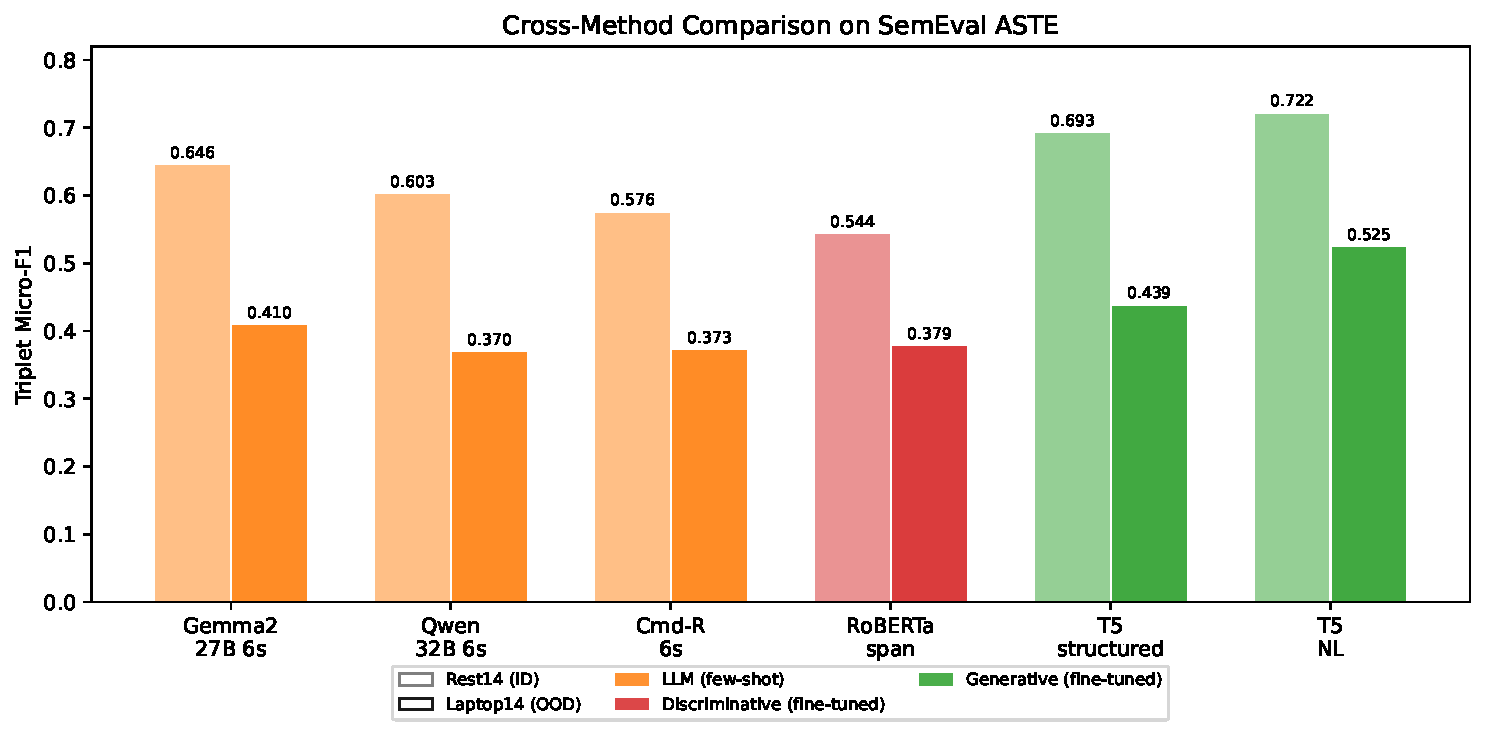
\includegraphics[width=0.95\textwidth]{figures/r4_crossmethod_english.pdf}
\caption{Cross-method comparison on SemEval ASTE: LLMs (few-shot) vs fine-tuned models, showing both in-domain (Rest14) and out-of-domain (Laptop14) performance.}
\label{fig:r4-crossmethod}
\end{figure}


\section{LLMs on Romanian ABSA}\label{sec:llm-romanian}

\begin{table}[H]
\centering
\caption{Romanian ABSA results on eMAG phone reviews. Pair F1 = polarity + category must both match.}
\label{tab:romanian}
\small
\begin{tabular}{@{}lrccc@{}}
\toprule
\textbf{Method} & \textbf{Params} & \textbf{Pair F1} & \textbf{Polarity F1} & \textbf{Category F1} \\
\midrule
\multicolumn{5}{l}{\textit{LLMs (few-shot, no fine-tuning)}} \\
\midrule
Gemma2 27B 0-shot & 27B & 0.745 & \textbf{0.888} & 0.804 \\
Gemma2 27B 6-shot & 27B & 0.758 & \textbf{0.888} & 0.826 \\
Qwen2.5 32B 0-shot & 32B & 0.621 & 0.854 & 0.689 \\
Qwen2.5 32B 6-shot & 32B & 0.740 & 0.881 & 0.807 \\
Command-R 0-shot & 35B & 0.535 & 0.766 & 0.612 \\
Command-R 6-shot & 35B & 0.750 & 0.880 & 0.821 \\
\midrule
\multicolumn{5}{l}{\textit{Fine-tuned models}} \\
\midrule
RoBERT-base (RO) & 114M & 0.792 & 0.878 & \textbf{0.862} \\
bert-base-ro-cased & 110M & 0.793 & 0.877 & 0.858 \\
XLM-R-base & 278M & \textbf{0.795} & 0.881 & 0.861 \\
FLAN-T5-base (NL) & 250M & 0.764 & 0.882 & 0.853 \\
\bottomrule
\end{tabular}
\end{table}

Polarity classification is easy for all methods (0.85--0.89 F1). The bottleneck is category prediction, where LLMs score 0.61--0.83 while fine-tuned models achieve 0.85--0.86. This makes sense: the category taxonomy (11 classes) is specific to this dataset and not something LLMs would have encountered during pre-training. The 6-shot demonstrations help LLMs learn the taxonomy (Command-R jumps from 0.61 to 0.82 in category F1 with examples), but they still fall short of fine-tuned models that have seen the full training set.

XLM-R-base (278M, multilingual) achieves the best pair F1 (0.795), followed closely by the two monolingual Romanian models: bert-base-romanian-cased (0.793) and RoBERT-base (0.792). FLAN-T5-base (0.764) trails slightly. All fine-tuned models outperform all LLMs on pair F1.

Gemma2 27B stands out in 0-shot: it achieves 0.745 pair F1 without any task-specific data, nearly matching the fine-tuned FLAN-T5. This suggests that Gemma2's multilingual pre-training included enough Romanian text to perform sentiment analysis competently. However, it still falls short on category prediction (0.804 vs 0.858--0.862 for fine-tuned models).

\begin{figure}[H]
\centering
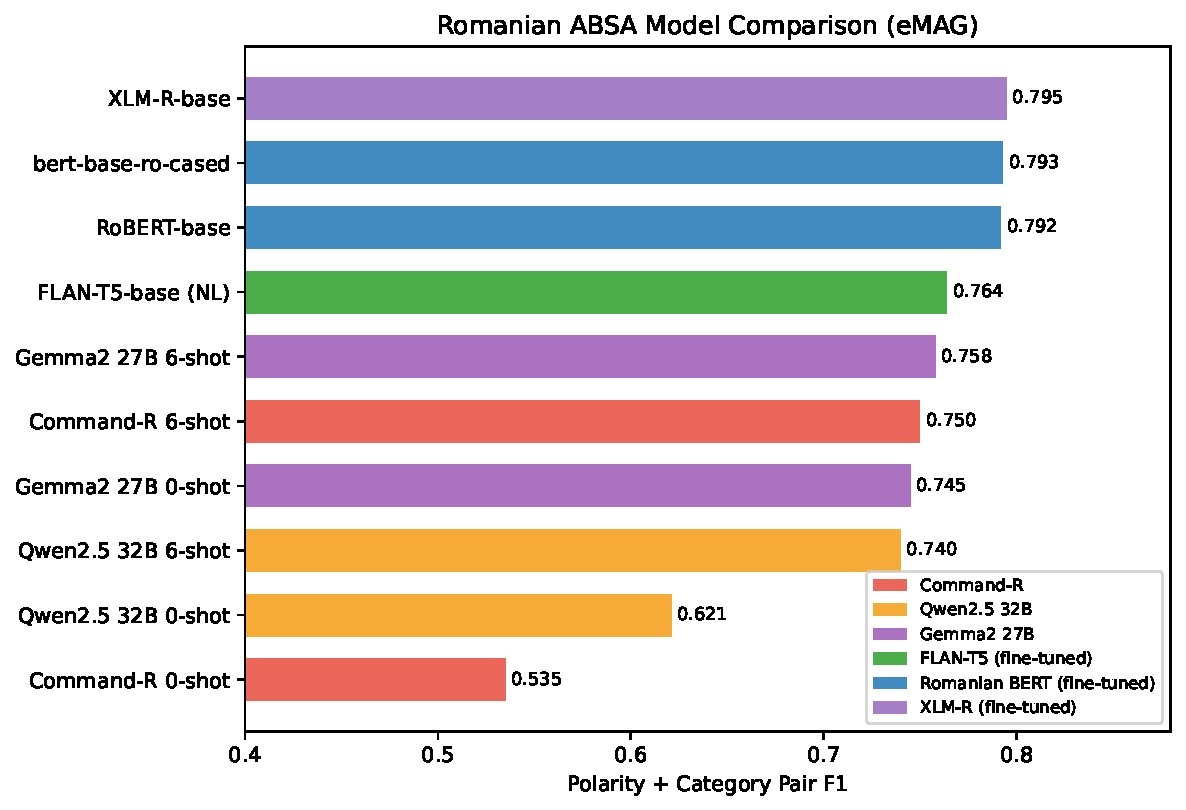
\includegraphics[width=0.85\textwidth]{figures/r4_romanian_comparison.pdf}
\caption{Romanian ABSA model comparison: all models ranked by polarity + category pair F1.}
\label{fig:r4-romanian}
\end{figure}

\begin{figure}[H]
\centering
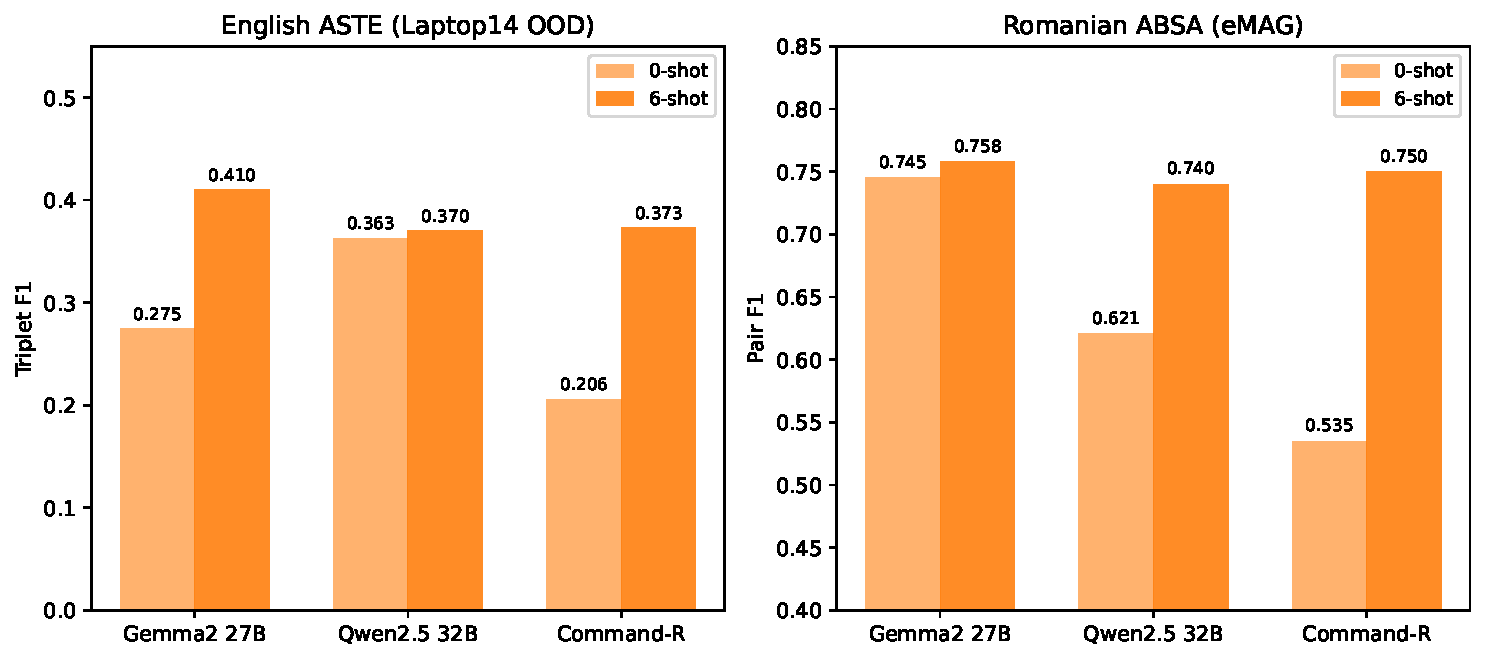
\includegraphics[width=0.95\textwidth]{figures/r4_llm_0shot_vs_6shot.pdf}
\caption{LLM performance in 0-shot vs 6-shot settings on English ASTE (left) and Romanian ABSA (right).}
\label{fig:r4-0vs6}
\end{figure}


\section{Discussion: Monolingual vs Multilingual Models}\label{sec:mono-vs-multi}

The Romanian experiments provide a direct comparison along the language specialisation axis:

\begin{itemize}
    \item RoBERT-base (114M, Romanian-only): 0.792 pair F1
    \item bert-base-romanian-cased (110M, Romanian-only): 0.793 pair F1
    \item XLM-R-base (278M, 100-language): 0.795 pair F1
    \item FLAN-T5-base (250M, English instruction-tuned): 0.764 pair F1
\end{itemize}

The monolingual Romanian models (110--114M) perform within 0.3 F1 points of XLM-R-base (278M) despite being 2.5$\times$ smaller. This is consistent with what Masala et al.~\cite{masala2020robert} and Dumitrescu et al.~\cite{dumitrescu2020birth} reported for POS tagging and NER: monolingual pre-training on dedicated Romanian corpora produces models that match or approach larger multilingual models on downstream tasks in that language.

This finding is not specific to Romanian. Velankar et al.~\cite{velankar2022mono} demonstrated the same pattern for Marathi: monolingual Marathi BERT models outperformed XLM-RoBERTa on five downstream tasks including text classification, despite the multilingual model being substantially larger. Hasan et al.~\cite{tanvir2023bangla} reported consistent findings for Bangla sentiment analysis, where monolingual transformer models outperformed multilingual alternatives even in few-shot scenarios. The pattern appears to be general: for a given downstream task in a specific language, a dedicated monolingual model matches or exceeds a larger multilingual model when sufficient monolingual pre-training data is available.

The explanation lies in what Conneau et al.~\cite{conneau2020unsupervised} acknowledged when introducing XLM-R and what subsequent work has termed the ``curse of multilinguality''~\cite{chang2023multilinguality, pfeiffer2024breaking}: as a fixed-capacity model covers more languages, per-language performance decreases because the model's parameters must simultaneously represent the structure of all languages. Bérard et al.~\cite{berard2026capacity} confirmed this empirically in 2026, showing that multilingual language models consistently underperform monolingual counterparts due to capacity constraints. XLM-R-base (278M parameters) distributes its capacity across 100 languages, meaning Romanian gets a fraction of the total representational budget. RoBERT-base (114M parameters) dedicates all its capacity to Romanian, having been trained on 12GB of exclusively Romanian text. The result is that per-parameter efficiency for Romanian is much higher in the monolingual model.

In our results, XLM-R does still slightly outperform the monolingual models (0.795 vs 0.792--0.793). This small advantage may come from cross-lingual transfer: XLM-R has seen sentiment-related patterns across many languages during pre-training, and some of these transfer to Romanian. The difference is small enough (0.2--0.3 F1 points) that it would likely disappear with multi-seed evaluation or reverse with slightly different hyperparameters. For practical purposes, the monolingual and multilingual models are equivalent on this task.

The practical implication is that for Romanian ABSA classification, a 110M monolingual model provides essentially the same performance as a 278M multilingual model at lower computational cost. This matters for deployment: the monolingual model is faster to fine-tune, requires less memory at inference, and achieves the same result. The additional capacity of XLM-R provides no meaningful benefit when target-language fine-tuning data is available.

FLAN-T5-base trails by 3 points despite being a 250M model. This is expected: it is an English-centric generative model being asked to perform a classification task in a language it was not primarily trained on. That it still achieves 0.764, outperforming all LLMs, demonstrates that even modest fine-tuning on target-language data is effective. But for this particular task (classification with a fixed taxonomy), the encoder-based classifiers with language-appropriate pre-training have a natural architectural advantage: they produce a single representation that feeds directly into classification heads, while the generative model must produce the correct output token by token, which is a harder problem for a model generating in an unfamiliar language.


\section{Discussion: Annotation Quality and Performance Ceiling}\label{sec:annotation}

Evaluating models on benchmark data assumes that the gold annotations represent ground truth. In practice, annotation is a subjective and error-prone process, and the degree of annotator agreement sets an upper bound on achievable performance. Miñarro-Giménez et al.~\cite{minarro2019quantitative} demonstrated this quantitatively for clinical text annotation: even trained annotators show non-trivial disagreement on structured labelling tasks, with error rates and inconsistencies that cannot be eliminated through guidelines alone. The implication is that any model evaluated against a single set of gold annotations is being measured against an imperfect standard.

This applies directly to ABSA. The SemEval datasets~\cite{pontiki2014semeval} were annotated by human annotators following task-specific guidelines, but the guidelines leave room for interpretation in cases involving implicit sentiment, pragmatic inference, and debatable polarity. In our error analysis on Laptop14 (detailed in our previous report), we identified several recurring patterns where the model's prediction is at least as defensible as the gold label:

\begin{itemize}
    \item Desire and requirement contexts: ``I needed a laptop with big storage'' is annotated as [storage, big, neutral], treating the desire context as non-opinionated. The model predicts positive because ``big'' is a positive-valence adjective in the vast majority of its training examples. Neither interpretation is clearly wrong; it depends on whether the annotation scheme prioritises surface lexical polarity or pragmatic speech-act intent.

    \item Missing-feature complaints: ``There is no HDMI receptacle'' is annotated as neutral. The model predicts negative, which aligns with how most readers would interpret a review statement about a missing feature. The neutral label follows from a strict reading of the guidelines (no explicit opinion word), but misses the implicit dissatisfaction.

    \item Hypothetical and counterfactual constructions: ``a spice rub might have overwhelmed'' is annotated as a negative opinion about spice rub, despite being a hypothetical dismissal (the reviewer is saying the chef avoided something bad). These require pragmatic reasoning that goes beyond what surface-level patterns can capture.
\end{itemize}

These cases connect to a broader issue in NLP: the distinction between surface semantics and implicit meaning. Li et al.~\cite{li2021implicit} showed that neural language models develop implicit representations of entity state and situation dynamics from text alone, but these representations are imperfect and incomplete. Sun et al.~\cite{sun2025implicit} argue more recently that text embedding research should move beyond capturing surface meaning toward modelling implicit semantics, precisely the kind of pragmatic inference needed to correctly handle the cases above. Our models, trained on surface-level aspect-opinion-polarity annotations, predictably struggle with cases where the correct label requires understanding speech acts, pragmatic implicature, or counterfactual reasoning.

The problem is compounded for the Romanian dataset. The eMAG training data was annotated with GPT-4 assistance: reviews were processed by GPT-4 to identify aspects and assign polarity and category labels, followed by human review. Aldeen et al.~\cite{aldeen2023chatgpt} found that LLM-generated annotations achieve competitive quality for sentiment classification tasks, but human annotators consistently outperform on tasks requiring nuanced contextual judgement. For our Romanian data specifically, this means:

\begin{itemize}
    \item Category assignment is the most annotation-sensitive component. The boundary between categories like ``experience'' and ``performance'', or ``design'' and ``durability'', requires domain expertise and subjective judgement that GPT-4 may resolve differently from a human annotator familiar with Romanian consumer electronics vocabulary.

    \item There is an inherent circularity concern: models are trained on LLM-annotated data and then compared against LLMs on test data from the same annotation pipeline. We mitigate this by using an independently annotated test set, but biases in the training set still propagate to all fine-tuned models.

    \item The quality ceiling is bounded by the annotation model's ability to perform fine-grained Romanian ABSA. Our evaluation shows that Gemma2 27B achieves approximately 0.75 pair F1 on this task in 0-shot, and GPT-4 (used for annotation) is likely somewhat better but not dramatically so on this specific Romanian task. Training data produced by an imperfect annotator, whether human or LLM, may contain systematic errors that limit all models trained on it.
\end{itemize}

The practical consequence is that reported F1 scores on both datasets should be interpreted with caution. The gap between model performance and ``perfect'' F1 is not entirely due to model limitations; a portion reflects genuine annotation ambiguity. Hu and Liu~\cite{hu2004mining}, in their early work on opinion mining, acknowledged that the task of identifying what constitutes an opinion and what is merely a factual statement is inherently subjective and context-dependent. Two decades later, this remains the fundamental challenge.

For the English SemEval data, we estimate that 5--10\% of Laptop14 annotations involve genuinely ambiguous polarity. For the Romanian data, the proportion may be higher due to the automated annotation pipeline, though we have not quantified it precisely. Importantly, this annotation noise affects all methods equally: relative comparisons between models remain valid even if absolute F1 scores overstate the difficulty of the underlying task.

On the English side, the LLM evaluation on SemEval is free from annotation circularity since the test data was annotated by humans independently. The LLMs' lower performance relative to fine-tuned models on this data reflects genuine capability differences in structured extraction rather than annotation artefacts.



\chapter{Conclusions}\label{ch:conclusions}

\section{Summary}

This report investigated two extensions of our previous work on generative ABSA: the comparison of fine-tuned models against large language models, and the application to Romanian as a representative medium-resource language.

On English ASTE, fine-tuned FLAN-T5-base (250M parameters) outperforms all tested LLMs (27--35B parameters) in both zero-shot and six-shot settings. The gap is 11.5 F1 points on out-of-domain data (Laptop14) between our best model and the best LLM. This is consistent with findings in the literature for structured extraction tasks: task-specific fine-tuning remains more effective than in-context learning at current LLM scales.

On Romanian ABSA, fine-tuned models (XLM-R, RoBERT, bert-ro, FLAN-T5) outperform LLMs on the combined polarity+category metric. Polarity classification is easy for all methods ($\sim$0.88 F1), while category prediction is the bottleneck for LLMs, particularly in 0-shot where the specific taxonomy is unknown to the model. Monolingual Romanian models (110--114M) perform within 0.3 F1 points of the 2.5$\times$ larger multilingual XLM-R, confirming that dedicated language-specific pre-training compensates for smaller model size on downstream tasks.

\section{Limitations}

\begin{itemize}
    \item LLM quantisation: all LLMs are 4-bit quantised, which reduces performance relative to full-precision inference. Results represent a lower bound on LLM capability.
    \item Single inference run: LLM evaluations use a single run (no temperature variation or multiple sampling). Variance is not characterised.
    \item Romanian dataset size: the eMAG training set is relatively small, which may advantage models that converge quickly (BERT-based classifiers) over generative models that typically need more data.
    \item GPT-4 annotation: the training data annotation quality is bounded by GPT-4's capabilities on Romanian text, which may introduce systematic biases.
\end{itemize}

\section{Future Work}

\begin{itemize}
    \item Fine-tuning smaller LLMs (7--8B parameters) on ABSA tasks, to find the scale at which fine-tuned LLMs begin to outperform fine-tuned smaller models.
    \item Testing chain-of-thought prompting for LLMs on extraction tasks, which might help with the span boundary identification problem.
    \item Expanding Romanian ABSA evaluation to other product categories (not just phones) and to triplet extraction (ASTE) rather than just polarity+category classification.
    \item Evaluating the effect of increasing few-shot examples (12-shot, 24-shot) to determine how much demonstration data LLMs need to approach fine-tuned performance.
\end{itemize}


\chapter{Annex}\label{ch:annex}

\section{LLM Prompt Templates}

\textbf{English ASTE (6-shot format):}
\begin{lstlisting}
Extract all (aspect, opinion, polarity) triplets from the sentence.
Polarity is one of: positive, negative, neutral.
Output format: [aspect, opinion, polarity]

Example 1:
Sentence: Great food but the service was dreadful !
Output: [food, Great, positive] [service, dreadful, negative]

... (5 more examples) ...

Sentence: {test_sentence}
Output:
\end{lstlisting}

\textbf{Romanian ABSA (6-shot format):}
\begin{lstlisting}
Extrageti perechi (polaritate, categorie) din recenzia data.
Polaritatea: positive, negative, neutral.
Categorii: experience, durability, performance, battery,
  price_quality, design, camera, audio, software, brand, service.

Exemplu 1:
Recenzie: Telefonul este rapid si bateria tine bine.
Output: [positive, performance] [positive, battery]

... (5 more examples) ...

Recenzie: {test_sentence}
Output:
\end{lstlisting}

\section{Per-Model LLM Results (English)}

\begin{table}[H]
\centering
\caption{Gemma2 27B detailed results (SemEval ASTE, triplet micro-F1).}
\small
\begin{tabular}{@{}lcccc@{}}
\toprule
\textbf{Setting} & \textbf{Rest14} & \textbf{Rest15} & \textbf{Rest16} & \textbf{Laptop14} \\
\midrule
0-shot & 0.441 & 0.418 & 0.455 & 0.275 \\
6-shot & 0.646 & 0.592 & 0.637 & 0.410 \\
\bottomrule
\end{tabular}
\end{table}

\begin{table}[H]
\centering
\caption{Qwen2.5 32B detailed results (SemEval ASTE, triplet micro-F1).}
\small
\begin{tabular}{@{}lcccc@{}}
\toprule
\textbf{Setting} & \textbf{Rest14} & \textbf{Rest15} & \textbf{Rest16} & \textbf{Laptop14} \\
\midrule
0-shot & 0.535 & 0.451 & 0.556 & 0.363 \\
6-shot & 0.603 & 0.527 & 0.614 & 0.370 \\
\bottomrule
\end{tabular}
\end{table}

\begin{table}[H]
\centering
\caption{Command-R detailed results (SemEval ASTE, triplet micro-F1).}
\small
\begin{tabular}{@{}lcccc@{}}
\toprule
\textbf{Setting} & \textbf{Rest14} & \textbf{Rest15} & \textbf{Rest16} & \textbf{Laptop14} \\
\midrule
0-shot & 0.318 & 0.256 & 0.309 & 0.206 \\
6-shot & 0.576 & 0.499 & 0.568 & 0.373 \\
\bottomrule
\end{tabular}
\end{table}


\clearpage
\addcontentsline{toc}{chapter}{Bibliography}
\bibliographystyle{ieeetr}
\bibliography{bibliography4}

\end{document}
